\section{CƠ SỞ LÝ THUYẾT}

Chương này trình bày toàn bộ nền tảng lý thuyết cốt lõi về Mô hình Mạng Zero Trust theo chuẩn NIST SP 800-207 và Khung trưởng thành 5 trụ cột CISA. Chương đi sâu phân tích sơ đồ kiến trúc tổng thể, mô tả chi tiết 5 luồng nghiệp vụ y tế cốt lõi (BF-01 đến BF-05) cùng ma trận phân quyền RBAC chi tiết. Đồng thời, chương giải thích cụ thể lý do tại sao lựa chọn và mục đích sử dụng của từng công nghệ trong hệ thống.

\subsection{Tổng quan về Mô hình Kiến trúc Zero Trust}

Kiến trúc Zero Trust dựa trên khung hướng dẫn NIST SP 800-207 thiết lập một nguyên tắc bảo mật căn bản là loại bỏ hoàn toàn niềm tin ngầm định theo vị trí kết nối vật lý. Dù người dùng truy cập từ mạng LAN nội bộ bệnh viện hay từ mạng Internet bên ngoài, mọi yêu cầu truy cập đều phải trải qua quá trình kiểm tra danh tính và cấp quyền liên tục.

Khung trưởng thành Zero Trust của Cơ quan An toàn An ninh mạng và Hạ tầng Mỹ (CISA) phân chia mô hình phòng thủ thành 5 trụ cột chính nhằm đảm bảo tính bao quát toàn diện bao gồm: Identity (Danh tính), Devices (Thiết bị), Networks (Mạng), Applications and Workloads (Ứng dụng) và Data (Dữ liệu), kết hợp với năng lực giám sát tập trung Visibility and Analytics.

\begin{figure}[H]
    \centering
    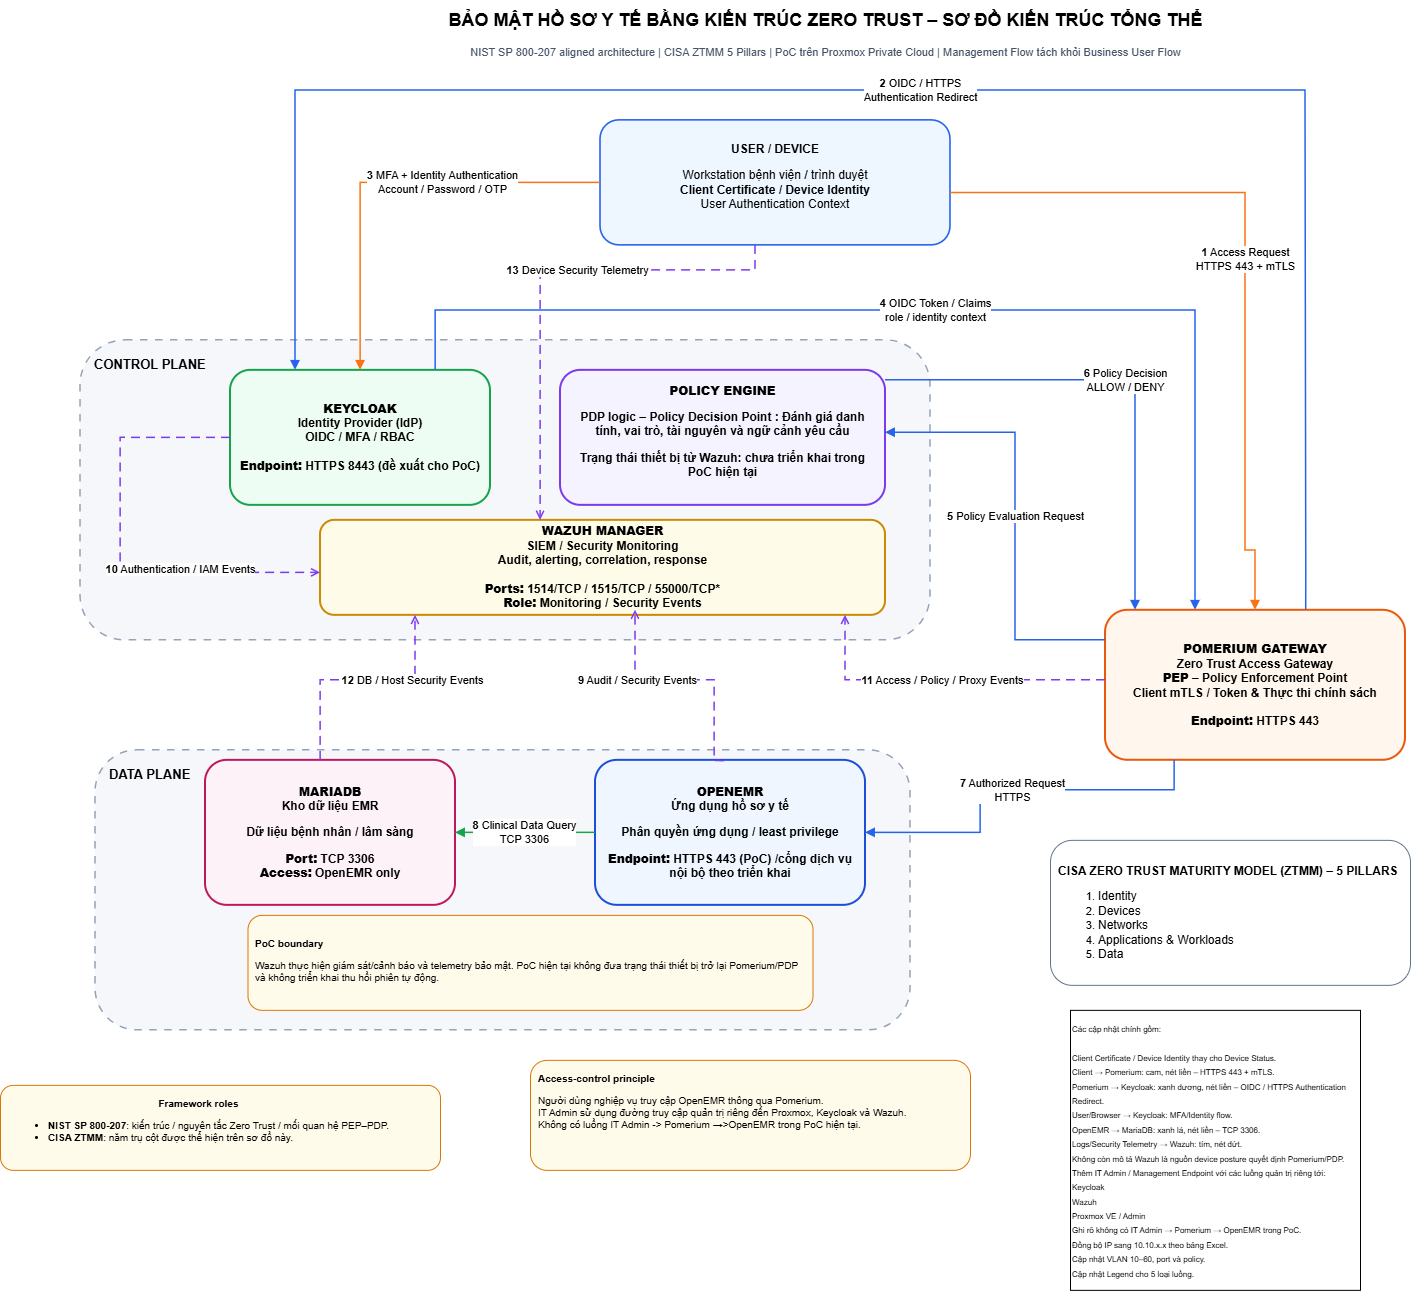
\includegraphics[width=0.95\textwidth]{image/zero_trust_overall_architecture_v2-Zero Trust Architecture.drawio.png}
    \caption{Sơ đồ kiến trúc tổng thể mô hình Zero Trust bảo mật Hồ sơ Y tế}
    \label{fig:overall_architecture}
\end{figure}

\subsubsection{Giải thích Chi tiết Sơ đồ Kiến trúc Tổng thể Mô hình Zero Trust (Hình 2.1)}

Sơ đồ kiến trúc tổng thể thể hiện mối quan hệ tương tác giữa 4 vùng thành phần chính: Vùng người dùng (Users/Devices), Vùng điều khiển truy cập (Access Control), Vùng ứng dụng \& dữ liệu (App \& Database), và Vùng giám sát an ninh (Security Monitoring).

Tạo tầng gác cổng uỷ quyền danh tính (Identity-Aware Proxy - Pomerium): Khi bác sĩ, kỹ thuật viên xét nghiệm hay nhân viên y tế truy cập từ thiết bị đầu cuối, luồng kết nối không đi trực tiếp vào máy chủ y tế mà bắt buộc phải trỏ tới Pomerium Access Gateway đóng vai trò Policy Enforcement Point (PEP). Pomerium kiểm tra chứng chỉ số cá thể (Client Certificate) được cài sẵn trên thiết bị thông qua giao thức mTLS để xác định thiết bị có thuộc danh sách được bệnh viện cấp phép hay không.

Tích hợp xác thực danh tính tập trung (Keycloak IdP): Khi kết nối mTLS hợp lệ, Pomerium chuyển hướng giao diện đăng nhập về Keycloak qua giao thức OIDC. Người dùng nhập tên tài khoản, mật khẩu và bắt buộc hoàn thành bước xác thực đa yếu tố (MFA) bằng việc nhập mã OTP từ ứng dụng Google Authenticator. Sau khi xác thực thành công, Keycloak trả về ID Token và Access Token chứa danh sách các vai trò (Roles) của người dùng.

Thực thi chính sách uỷ quyền ngữ cảnh (Policy Decision Point - PDP): Pomerium tiếp nhận Token từ Keycloak và đối chiếu với tập quy tắc Policy Route. Nếu vai trò của người dùng khớp với quyền hạn được phép truy cập tài nguyên y tế tương ứng, Pomerium mới khởi tạo kết nối uỷ quyền bảo mật (Authorized HTTPS) đưa lưu lượng vào ứng dụng OpenEMR. Các kết nối không đủ điều kiện xác thực hoặc sai vai trò sẽ bị Pomerium ra quyết định Deny và ngắt kết nối lập tức.

Bảo vệ vùng ứng dụng OpenEMR và cơ sở dữ liệu MariaDB: Máy chủ OpenEMR tiếp nhận luồng dữ liệu từ Pomerium và thực hiện phân quyền chi tiết RBAC ở tầng ứng dụng. Cơ sở dữ liệu MariaDB nằm ở phân đoạn mạng cô lập sâu nhất, chỉ chấp nhận kết nối duy nhất đến từ OpenEMR qua cổng TCP 3306. Dữ liệu trên MariaDB được mã hóa cấu trúc lưu trữ TDE (Encryption at Rest), đảm bảo an toàn tuyệt đối ngay cả khi tệp tin dữ liệu thô bị trích xuất ngoài ý muốn.

Tập trung giám sát an ninh và ghi nhận nhật ký (Wazuh SIEM/XDR): Tất cả các thành phần từ Pomerium, Keycloak, OpenEMR, MariaDB cho đến các máy ảo hạ tầng đều được cài đặt Wazuh Agent. Các nhật ký sự kiện (security events), nhật ký truy cập, cảnh báo đăng nhập thất bại và sự kiện thay đổi tệp tin cấu hình (FIM) đều được truyền liên tục về Wazuh Manager để phục vụ giám sát thời gian thực, phát cảnh báo và hỗ trợ truy vết an ninh.

\begingroup
\setlength\LTleft{0pt}
\setlength\LTright{0pt}
\begin{longtable}{| >{\raggedright\arraybackslash}p{3.2cm} | >{\raggedright\arraybackslash}p{5.5cm} | >{\raggedright\arraybackslash}p{5.5cm} |}
\caption{Bảng đối chiếu các công nghệ mã nguồn mở đáp ứng 5 trụ cột Zero Trust} \label{tab:cisa_mapping} \\
\hline
\textbf{Trụ cột / Năng lực} & \textbf{Tiêu chí bảo mật theo CISA} & \textbf{Công nghệ triển khai} \\ \hline
\endhead
\hline
\endfoot

Identity (Danh tính) & Xác thực người dùng, MFA, SSO, quản lý vai trò và phiên làm việc & Keycloak + Pomerium \\ \hline
Devices (Thiết bị) & Nhận diện thiết bị tin cậy, mTLS và theo dõi security posture & Client Certificate + mTLS + Wazuh Agent \\ \hline
Networks (Mạng) & Phân đoạn mạng logic, loại bỏ implicit trust, ngăn lateral movement & Proxmox VE Firewall + 6 VLANs + Pomerium Gateway \\ \hline
Applications \& Workloads & Bảo vệ ứng dụng OpenEMR, kiểm soát quyền truy cập theo context & Pomerium Policy + OpenEMR RBAC \\ \hline
Data (Dữ liệu) & Mã hóa đường truyền end-to-end và mã hóa dữ liệu lưu trữ tại ổ đĩa & TLS/HTTPS + MariaDB TDE Encryption \\ \hline
Visibility \& Analytics & Thu thập log tập trung, giám sát tính toàn vẹn và cảnh báo sự cố & Wazuh SIEM/XDR Manager + Agent \\ \hline
\end{longtable}
\endgroup

\subsection{Luồng Hoạt động Nghiệp vụ và Ma trận Phân quyền Chi tiết}

\subsubsection{Phân tích các Luồng Hoạt động Nghiệp vụ Cốt lõi (BF-01 đến BF-05)}

Dựa trên quy trình khám chữa bệnh và quản lý hồ sơ tại cơ sở y tế, hệ thống xác định năm luồng nghiệp vụ cốt lõi. Các luồng này thể hiện quá trình từ khi bệnh nhân được tiếp nhận, khám bệnh, thực hiện xét nghiệm cho đến khi hồ sơ bệnh án được lưu trữ, khai thác và phân công quản lý.

\textbf{Luồng nghiệp vụ BF-01 (Tiếp nhận bệnh nhân và tạo lượt khám):}
Nhân viên Lễ tân thực hiện tìm kiếm thông tin bệnh nhân trên hệ thống. Đối với bệnh nhân đã có hồ sơ, Lễ tân kiểm tra và cập nhật các thông tin hành chính cần thiết. Đối với bệnh nhân mới, Lễ tân nhập thông tin cá nhân để tạo hồ sơ bệnh nhân. Sau khi hoàn tất quá trình tiếp nhận, Lễ tân tạo lượt khám mới và ghi nhận các thông tin phục vụ việc khám bệnh. Phạm vi công việc của Lễ tân tập trung vào hoạt động tiếp nhận và quản lý thông tin hành chính của bệnh nhân, không bao gồm việc cập nhật các nội dung chuyên môn như chẩn đoán hoặc ghi chú lâm sàng.

\textbf{Luồng nghiệp vụ BF-02 (Khám bệnh, ghi chú lâm sàng và chẩn đoán):}
Sau khi bệnh nhân được tiếp nhận và tạo lượt khám, Bác sĩ tiến hành mở hồ sơ bệnh nhân để xem các thông tin cần thiết phục vụ quá trình khám. Bác sĩ thực hiện khám lâm sàng, ghi nhận triệu chứng, tiền sử liên quan, cập nhật ghi chú diễn biến và đưa ra chẩn đoán. Trong trường hợp cần thêm thông tin hỗ trợ chẩn đoán, Bác sĩ có thể tạo chỉ định xét nghiệm hoặc các dịch vụ cận lâm sàng phù hợp. Sau khi có đầy đủ thông tin, Bác sĩ tiếp tục cập nhật nội dung chuyên môn và hoàn thiện quá trình khám bệnh. Bác sĩ chỉ được cập nhật các nội dung chuyên môn đối với bệnh nhân và lượt khám thuộc phạm vi được phân công phụ trách; việc thay đổi thông tin chuyên môn của các lượt khám ngoài phạm vi phụ trách không được phép thực hiện. Trong trường hợp bệnh nhân cần tiếp tục điều trị nội trú, Bác sĩ có thể thực hiện chuyển bệnh nhân sang trạng thái nhập viện theo phạm vi nghiệp vụ của hệ thống. Quyền cập nhật hồ sơ nội trú sau đó chỉ áp dụng đối với Bác sĩ được phân công phụ trách bệnh nhân tương ứng.

\textbf{Luồng nghiệp vụ BF-03 (Chỉ định và xử lý kết quả xét nghiệm):}
Trong quá trình khám bệnh, khi cần thực hiện xét nghiệm, Bác sĩ tạo chỉ định xét nghiệm cho bệnh nhân. Kỹ thuật viên xét nghiệm tiếp nhận chỉ định, thực hiện xét nghiệm và cập nhật kết quả tương ứng. Trong thời gian xét nghiệm chưa hoàn tất, chỉ định có thể được điều chỉnh theo yêu cầu nghiệp vụ. Sau khi xét nghiệm đã hoàn thành và có kết quả, nội dung chỉ định liên quan không được thay đổi nhằm bảo đảm tính nhất quán giữa yêu cầu xét nghiệm và kết quả đã thực hiện. Sau khi kết quả xét nghiệm được xác nhận, Kỹ thuật viên xét nghiệm không được tiếp tục chỉnh sửa kết quả đó. Bác sĩ sử dụng kết quả đã xác nhận để hỗ trợ quá trình đánh giá tình trạng bệnh và hoàn thiện chẩn đoán.

\textbf{Luồng nghiệp vụ BF-04 (Khai thác hồ sơ bệnh án):}
Sau khi các thông tin khám bệnh được hình thành trong quá trình điều trị, hồ sơ bệnh án được lưu trữ để phục vụ nhu cầu quản lý và khai thác sau này. Nhân viên quản lý hồ sơ tiếp nhận các hồ sơ được phân công và thực hiện tra cứu thông tin bệnh nhân, lịch sử khám bệnh, tài liệu và các nội dung liên quan phục vụ nghiệp vụ quản lý hồ sơ. Nhân viên chỉ thực hiện khai thác những hồ sơ thuộc phạm vi công việc được giao và không tham gia chỉnh sửa các nội dung chuyên môn do Bác sĩ hoặc các bộ phận chuyên môn khác tạo ra.

\textbf{Luồng nghiệp vụ BF-05 (Phân công và chuyển giao hồ sơ bệnh án):}
Để quản lý phạm vi khai thác hồ sơ giữa các nhân viên, Medical Records Supervisor thực hiện phân công bệnh nhân hoặc hồ sơ bệnh án cho từng nhân viên quản lý hồ sơ. Sau khi được phân công, nhân viên quản lý hồ sơ chịu trách nhiệm khai thác các hồ sơ tương ứng phục vụ công việc. Khi có thay đổi về nhân sự hoặc yêu cầu nghiệp vụ, Medical Records Supervisor có thể chuyển giao hồ sơ từ nhân viên đang phụ trách sang một nhân viên khác. Sau khi quá trình chuyển giao hoàn tất, nhân viên mới tiếp nhận trách nhiệm quản lý hồ sơ theo phân công mới. Luồng nghiệp vụ này giúp xác định rõ trách nhiệm của từng nhân viên đối với từng nhóm hồ sơ bệnh án và hạn chế việc khai thác hồ sơ ngoài phạm vi công việc được giao.

\subsubsection{Ma trận Phân quyền Chi tiết (Granular Role-Permission Matrix)}

Ma trận phân quyền dưới đây quy định chi tiết các quyền thao tác gồm Đọc, Tạo, Sửa, Xóa và Xuất đối với từng loại tài nguyên trong hệ thống, dành cho 6 nhóm vai trò nghiệp vụ gồm Lễ tân, Bác sĩ, Kỹ thuật viên xét nghiệm, Nhân viên quản lý hồ sơ, Giám sát hồ sơ và Quản trị viên CNTT. Một số quyền chỉ được thực hiện khi thỏa mãn các điều kiện nghiệp vụ như bệnh nhân/lượt khám thuộc phạm vi phụ trách, hồ sơ đã được phân công thông qua Medical Records Assignment hoặc trạng thái xử lý của xét nghiệm.

\begin{landscape}

\begingroup
\small
\setlength{\tabcolsep}{3pt}
\renewcommand{\arraystretch}{1.15}
\setlength\LTleft{0pt}
\setlength\LTright{0pt}

\begin{longtable}{|
>{\raggedright\arraybackslash}p{2.3cm} |
>{\raggedright\arraybackslash}p{2.8cm} |
>{\centering\arraybackslash}p{1.1cm} |
>{\centering\arraybackslash}p{1.1cm} |
>{\centering\arraybackslash}p{1.1cm} |
>{\centering\arraybackslash}p{1.1cm} |
>{\centering\arraybackslash}p{1.2cm} |
>{\raggedright\arraybackslash}p{8.0cm} |
}

\caption{Ma trận phân quyền chi tiết Role-Permission Matrix trong hệ thống y tế}
\label{tab:rbac_granular_matrix} \\

\hline
\textbf{Vai trò} &
\textbf{Tài nguyên} &
\textbf{Đọc} &
\textbf{Tạo} &
\textbf{Sửa} &
\textbf{Xóa} &
\textbf{Xuất} &
\textbf{Điều kiện / Ghi chú nghiệp vụ} \\
\hline
\endfirsthead

\hline
\textbf{Vai trò} &
\textbf{Tài nguyên} &
\textbf{Đọc} &
\textbf{Tạo} &
\textbf{Sửa} &
\textbf{Xóa} &
\textbf{Xuất} &
\textbf{Điều kiện / Ghi chú nghiệp vụ} \\
\hline
\endhead

\hline
\endfoot

% ===================== LỄ TÂN =====================

Lễ tân &
Thông tin hành chính &
Có & Có & Có & Không & Không &
Chỉ xử lý các thông tin hành chính phục vụ quá trình tiếp nhận bệnh nhân. \\
\hline

Lễ tân &
Lượt khám &
Có & Có & Không & Không & Không &
Được tạo lượt khám mới khi tiếp nhận bệnh nhân; không được chỉnh sửa hoặc xóa dữ liệu chuyên môn của lượt khám. \\
\hline

Lễ tân &
Chẩn đoán &
Không & Không & Không & Không & Không &
Không thuộc phạm vi nghiệp vụ của Lễ tân. \\
\hline

Lễ tân &
Kết quả xét nghiệm &
Không & Không & Không & Không & Không &
Không thuộc phạm vi nghiệp vụ của Lễ tân. \\
\hline


% ===================== BÁC SĨ =====================

Bác sĩ &
Hồ sơ bệnh án &
Có & Không & Không & Không & Không &
Được đọc thông tin bệnh án phục vụ hoạt động khám và điều trị trong phạm vi được phép. \\
\hline

Bác sĩ &
Ghi chú lâm sàng &
Có & Có* & Có* & Không & Không &
Chỉ được tạo hoặc sửa đối với bệnh nhân và lượt khám thuộc phạm vi được phân công phụ trách. \\
\hline

Bác sĩ &
Chẩn đoán &
Có & Có* & Có* & Không & Không &
Chỉ được tạo hoặc sửa chẩn đoán đối với bệnh nhân và lượt khám thuộc phạm vi được phân công phụ trách. \\
\hline

Bác sĩ &
Chỉ định xét nghiệm &
Có & Có* & Có* & Không & Có* &
Được tạo chỉ định cho bệnh nhân thuộc phạm vi phụ trách. Chỉ được thay đổi nội dung chỉ định trước khi xét nghiệm được thực hiện và có kết quả. \\
\hline

Bác sĩ &
Kết quả xét nghiệm &
Có & Không & Không & Không & Không &
Được đọc kết quả xét nghiệm phục vụ chẩn đoán; không được tạo hoặc chỉnh sửa kết quả do bộ phận xét nghiệm phụ trách. \\
\hline


% ===================== KỸ THUẬT VIÊN XÉT NGHIỆM =====================

KTV Xét nghiệm &
Chỉ định xét nghiệm &
Có* & Không & Có* & Không & Không &
Được tiếp nhận chỉ định thuộc phạm vi xử lý và cập nhật trạng thái xử lý; không được thay đổi nội dung chỉ định do Bác sĩ tạo. \\
\hline

KTV Xét nghiệm &
Kết quả xét nghiệm &
Có* & Có* & Có* & Không & Có* &
Được nhập và cập nhật kết quả xét nghiệm thuộc phạm vi xử lý. Sau khi kết quả đã được xác nhận thì không được tiếp tục chỉnh sửa. \\
\hline

KTV Xét nghiệm &
Chẩn đoán &
Không & Không & Không & Không & Không &
Không thuộc phạm vi nghiệp vụ xét nghiệm. \\
\hline

KTV Xét nghiệm &
Ghi chú lâm sàng &
Không & Không & Không & Không & Không &
Không thuộc phạm vi nghiệp vụ xét nghiệm. \\
\hline


% ===================== NHÂN VIÊN QUẢN LÝ HỒ SƠ =====================

Quản lý hồ sơ &
Hồ sơ bệnh án &
Có* & Không & Không & Không & Có* &
Chỉ được đọc hoặc trích xuất khi bệnh nhân/hồ sơ đang được phân công cho chính nhân viên đó thông qua Medical Records Assignment. \\
\hline

Quản lý hồ sơ &
Tài liệu y tế &
Có* & Có* & Có* & Không & Có* &
Chỉ xử lý tài liệu thuộc bệnh nhân/hồ sơ đang được phân công; không được chỉnh sửa nội dung chuyên môn do Bác sĩ hoặc bộ phận chuyên môn tạo ra. \\
\hline

Quản lý hồ sơ &
Chẩn đoán &
Có* & Không & Không & Không & Không &
Chỉ được đọc khi bệnh nhân/hồ sơ đang được phân công; không được tạo, sửa hoặc xóa chẩn đoán. \\
\hline

Quản lý hồ sơ &
Ghi chú lâm sàng &
Có* & Không & Không & Không & Không &
Chỉ được đọc khi bệnh nhân/hồ sơ đang được phân công; không được tạo, sửa hoặc xóa ghi chú lâm sàng. \\
\hline

Quản lý hồ sơ &
Kết quả xét nghiệm &
Có* & Không & Không & Không & Không &
Chỉ được đọc khi bệnh nhân/hồ sơ đang được phân công; không được chỉnh sửa kết quả xét nghiệm. \\
\hline

Quản lý hồ sơ &
Thông tin phân công &
Có* & Không & Không & Không & Không &
Chỉ được xem thông tin phân công liên quan đến phạm vi của chính mình; không được tự assign hoặc reassign hồ sơ. \\
\hline


% ===================== GIÁM SÁT HỒ SƠ =====================

Giám sát hồ sơ &
Thông tin phân công &
Có & Có & Có & Không & Không &
Được thực hiện assign và reassign bệnh nhân/hồ sơ cho Nhân viên quản lý hồ sơ. \\
\hline

Giám sát hồ sơ &
Thông tin hành chính &
Có* & Không & Không & Không & Không &
Chỉ được xem các thông tin tối thiểu cần thiết để xác định đúng bệnh nhân khi thực hiện phân công hồ sơ. \\
\hline

Giám sát hồ sơ &
Dữ liệu chuyên môn &
Không & Không & Không & Không & Không &
Quyền quản lý việc phân công hồ sơ không đồng nghĩa với quyền truy cập hoặc chỉnh sửa nội dung chuyên môn của bệnh án. \\
\hline


% ===================== IT ADMIN =====================

IT Admin &
Tài khoản / Role &
Có & Có & Có & Không & Không &
Quản lý tài khoản và vai trò người dùng; khi tài khoản không còn được sử dụng thì thực hiện vô hiệu hóa thay vì xóa. \\
\hline

IT Admin &
Bảo mật / Log &
Có & Không & Có & Không & Không &
Thực hiện các thao tác quản trị kỹ thuật và cấu hình bảo mật trong phạm vi được cấp. \\
\hline

IT Admin &
Hồ sơ bệnh án &
Không & Không & Không & Không & Không &
Quyền quản trị hệ thống không mặc định đồng nghĩa với quyền đọc hoặc chỉnh sửa nội dung hồ sơ bệnh án. \\
\hline

\end{longtable}

\endgroup

\end{landscape}

\noindent\textit{Ghi chú quy ước trong bảng:}
\begin{itemize}
    \item \textbf{Có}: Quyền được cấp theo vai trò.
    \item \textbf{Có*}: Quyền được cấp có điều kiện; phải thỏa mãn ràng buộc tại cột ``Điều kiện / Ghi chú nghiệp vụ''.
    \item \textbf{Không}: Quyền không được cấp.
\end{itemize}

\subsection{Chi tiết các Công nghệ Triển khai và Lý do Lựa chọn}

\subsubsection{Hệ thống Quản lý Danh tính tập trung Keycloak}

\textbf{Tại sao lựa chọn sử dụng Keycloak:} Keycloak là giải pháp Quản lý Danh tính và Truy cập (IAM/IdP) mã nguồn mở hàng đầu hiện nay, hỗ trợ đầy đủ các chuẩn xác thực hiện đại như OIDC, OAuth 2.0 và SAML 2.0, có khả năng mở rộng cao và tích hợp dễ dàng với các dịch vụ uỷ quyền.

\textbf{Mục đích sử dụng cụ thể:} Keycloak được dùng làm máy chủ Identity Provider (IdP) trung tâm cho toàn bộ hệ thống y tế. Keycloak đảm nhận nhiệm vụ lưu trữ tài khoản người dùng, quản lý vai trò (Role-Based Access Control - RBAC), bắt buộc người dùng thực hiện xác thực đa yếu tố (MFA qua Google Authenticator/OTP) và cung cấp cơ chế Đăng nhập một lần (SSO) cho toàn bộ nhân viên y tế.

\subsubsection{Cổng Uỷ quyền Nhận biết Danh tính Pomerium (Identity-Aware Proxy)}

\textbf{Tại sao lựa chọn sử dụng Pomerium:} Pomerium là giải pháp Access Proxy độc lập hoạt động theo kiến trúc Zero Trust (ZTNA), cho phép kiểm tra quyền truy cập ở cấp độ HTTP/HTTPS request dựa trên danh tính người dùng được trả về từ IdP mà không cần cài đặt VPN client phức tạp.

\textbf{Mục đích sử dụng cụ thể:} Pomerium đóng vai trò là trạm gác Policy Enforcement Point (PEP) đứng trước hệ thống y tế. Mọi luồng truy cập của bác sĩ, kỹ thuật viên xét nghiệm, nhân viên y tế hay quản trị viên từ bên ngoài hoặc mạng nội bộ bắt buộc phải đi qua Pomerium. Pomerium sẽ liên kết với Keycloak qua OIDC để xác thực danh tính, kiểm tra chứng chỉ thiết bị (mTLS) và áp dụng các chính sách Allow/Deny định tuyến truy cập vào ứng dụng.

\subsubsection{Hệ thống Hồ sơ Y tế Điện tử OpenEMR}

\textbf{Tại sao lựa chọn sử dụng OpenEMR:}  
OpenEMR là phần mềm quản lý phòng khám và hồ sơ sức khỏe điện tử mã nguồn mở, cung cấp nhiều chức năng nghiệp vụ y tế như quản lý thông tin bệnh nhân, lượt khám, ghi chú lâm sàng, chẩn đoán, chỉ định xét nghiệm và kết quả xét nghiệm. OpenEMR đồng thời hỗ trợ cơ chế phân quyền theo vai trò và có khả năng tùy biến, phù hợp để xây dựng môi trường thử nghiệm cho các yêu cầu kiểm soát truy cập trong kiến trúc Zero Trust. OpenEMR hiện cũng có phiên bản được chứng nhận theo chương trình ONC Certified Health IT. 

\textbf{Mục đích sử dụng cụ thể:}  
OpenEMR được sử dụng làm hệ thống quản lý hồ sơ y tế trung tâm trong mô hình thử nghiệm. Nhóm xây dựng và kiểm thử các vai trò gồm Lễ tân, Bác sĩ, Kỹ thuật viên xét nghiệm, Nhân viên quản lý hồ sơ, Giám sát hồ sơ và Quản trị viên CNTT; đồng thời áp dụng ACL/GACL để kiểm soát chức năng của từng vai trò. Đối với nghiệp vụ quản lý hồ sơ, cơ chế Medical Records Assignment được bổ sung để giới hạn Nhân viên quản lý hồ sơ chỉ được truy cập những bệnh nhân đã được phân công, trong khi Giám sát hồ sơ thực hiện việc phân công hoặc chuyển giao hồ sơ.

\subsubsection{Hệ quản trị Cơ sở Dữ liệu MariaDB và Cơ chế Mã hóa Dữ liệu Lưu trữ}

\textbf{Tại sao lựa chọn sử dụng MariaDB TDE:} MariaDB là hệ quản trị cơ sở dữ liệu quan hệ mạnh mẽ, tương thích hoàn toàn với OpenEMR và tích hợp sẵn tính năng mã hóa dữ liệu trong suốt Transparent Data Encryption (TDE) thông qua plugin \url{file_key_management}.

\textbf{Mục đích sử dụng cụ thể:} MariaDB đảm nhận vai trò lưu trữ toàn bộ dữ liệu cơ sở của OpenEMR. Dự án kích hoạt cơ chế Data-at-Rest Encryption trên MariaDB để mã hóa toàn bộ các tệp tin lưu trữ dữ liệu (.ibd) trên ổ đĩa vật lý. Điều này đảm bảo nếu kẻ tấn công lấy cắp được ổ cứng vật lý hoặc tệp tin dữ liệu thô cũng không thể đọc được thông tin bệnh nhân nếu không có khóa master key.

\subsubsection{Hệ thống Cấp phát Chứng chỉ Easy-RSA và Xác thực Thiết bị mTLS}

\textbf{Tại sao lựa chọn sử dụng Easy-RSA và mTLS:} Easy-RSA là công cụ quản lý hạ tầng khóa công khai (PKI) nhỏ gọn, đáng tin cậy. Giao thức Mutual TLS (mTLS) cho phép xác thực hai chiều giữa client và server thông qua chứng chỉ số X.509 mà không thể bị giả mạo bởi địa chỉ IP hay MAC.

\textbf{Mục đích sử dụng cụ thể:} Easy-RSA được sử dụng để khởi tạo một Certificate Authority (CA) nội bộ cho hệ thống. CA này phát hành các chứng chỉ số cá thể (Client Certificates) cài đặt lên các thiết bị đầu cuối được bệnh viện cấp phép. Pomerium sẽ cấu hình mTLS bắt buộc; các thiết bị truy cập nếu không sở hữu chứng chỉ số hợp lệ do CA nội bộ cấp sẽ bị từ chối truy cập ngay tại tầng giao vận TLS.

\subsubsection{Hệ thống Giám sát An ninh Điểm cuối Wazuh SIEM/XDR}

\textbf{Tại sao lựa chọn sử dụng Wazuh:} Wazuh là nền tảng giám sát an ninh mạng và bảo vệ điểm cuối mã nguồn mở mạnh mẽ, cung cấp khả năng phát hiện đe dọa, giám sát tính toàn vẹn của tệp tin (FIM) và thu thập log tập trung theo thời gian thực.

\textbf{Mục đích sử dụng cụ thể:} Wazuh Agent được cài đặt lên tất cả các máy chủ ảo (VM) và thiết bị người dùng, truyền dữ liệu về Wazuh Manager tập trung. Wazuh đảm nhận nhiệm vụ giám sát sự thay đổi của các tệp tin cấu hình hệ thống, phát hiện các hành vi vô hiệu hóa tường lửa, ghi nhận các nỗ lực đăng nhập thất bại và phát cảnh báo tức thì cho quản trị viên an ninh.

\subsubsection{Nền tảng Ảo hóa Proxmox VE và Cơ chế Phân đoạn Mạng Logic}

\textbf{Tại sao lựa chọn sử dụng Proxmox VE:} Proxmox Virtual Environment (VE) là nền tảng ảo hóa doanh nghiệp mã nguồn mở tích hợp sẵn công nghệ Linux Bridge VLAN-aware và Proxmox Firewall, cho phép quản lý linh hoạt hạ tầng ảo và phân đoạn mạng an toàn.

\textbf{Mục đích sử dụng cụ thể:} Proxmox VE được sử dụng làm hạ tầng Hypervisor lưu trữ toàn bộ các máy chủ ảo của dự án. Proxmox VE cấu hình cầu nối VLAN-aware bridge (`vmbr1`) chia hệ thống thành 6 phân đoạn VLAN logic (Client, DMZ, Security, App, DB, Management). Proxmox Firewall được áp dụng để chặn toàn bộ kết nối trực tiếp từ người dùng vào máy chủ App và DB, bắt buộc mọi kết nối phải đi qua cổng Pomerium Proxy.
